\chapter{INTRODUCTION}
\label{chap:introduction}

Mobile computing is the preferred method of personal computing
environments for millions of users.
%
Furthermore, the mobile device market has grown over 400 million smartphones shipped
in 2011 and an estimated prediction of 1 billion shipments for
2015~\cite{dignan}.
%
This growth has been inspired by the hundreds of thousands of mobile
applications such as social networking, location-based services, image
processing, augmented reality, face and speech recognition.
%
In order to meet the increasing demands of these computationally-intense
applications, mobile platforms have been augmented with multi-core CPUs,
more powerful GPUs and other specialized hardware accelerators.
%
Despite of these many enhancements to the mobile platform's hardware,
however, the inescapable fact is that their limited batteries will
always serve as a bottleneck while hindering the mobile platforms from
utilizing their computing capabilities.\\
%
To address this issue, there have been research efforts in two different
areas: 1) heterogeneous computing and 2) computation offloading.
%
Heterogeneous computing has been seen as a mechanism to increase the
dynamic range of executions by dynamically combining computing elements
of various power performance characteristics and opportunistically scheduling the
workloads onto the optimal computing element based on the workload
requirements and energy availability~\cite{chen}.
%
Heterogeneous architectures with big/small cores, CPU/GPU and
CPU/hardware accelerators are now being offered by leading processor/SoC
vendors~\cite{bigprocessing, tegra}.
%
By allowing the dynamic workloads assignment onto the best processing
element based on the requirements, these architectures provide a wide
dynamic range of executions while improving performance when needed and
optimizing for energy performance.\\
%
In addition, computation offloading has been proposed as an alternative
for extending the capabilities of mobile platforms.
%
Since mobile networks have less throughput, and can exhibit higher
latencies and variances, computation offloading in mobile environments
is more constrained than previously studied cyber-foraging~\cite{cyber}
techniques in traditional computing systems.
%
In the past few years, there have been various mobile offloading
techniques proposed in the context of constrained mobile environments,
from application partitioning~\cite{maui} or process
migration~\cite{hung} to full mobile environment
cloning~\cite{clonecloud}.
%
Other works have also explored the implications of offloading to
different environments including the public cloud (i.e. Amazon
EC2)~\cite{hung}, to within private networks~\cite{shigeru}, and even to
other mobile devices~\cite{serendipity}.
%
All of these efforts seek for intelligent ways to enable mobile device
developers to leverage the computing capabilities of more powerful
external computing resources over the network.
%
Even though existing approaches provide core mechanisms to transform
typical mobile applications to offloading-enabled applications through
various granularities of partitioning and/or migration, they still lack
considerations for service discovery mechanisms while assuming the
availability of remote computing nodes with static endpoints.
%
Moreover, they have not investigated data privacy and secure
communication between the mobile client and remote resources, which can
be a crucial flaw for mobile computing environments.\\
%
This dissertation presents a novel framework which addresses the challenge
of remote computation offloading to resources in the cloud through the
paradigm of extended hardware-layer heterogeneous computing.
%
Heterogeneous computing uses specialized hardware accelerators to
increase computing throughput and performance.
%
I combine the power of cloud offloading with the flexibility of
heterogeneous architectures to provide an end-to-end heterogeneous
architecture which expands the dynamic execution range of mobile
platforms, which are typically limited in available energy resources.
%
For example, many data centers and public cloud providers are
integrating GPUs in their structure~\cite{bowman}, and software
designers are able to get better processing performance by offloading
more computation to the on-board GPUs than the CPUs.
%
Heterogeneous computing is not just restricted to the data center or to
cloud providers, it is also available in most personal computing
devices (i.e. workstations, laptops, and mobile devices) of the common
user.
%
Some examples are web browsers utilizing GPUs on a user's machine for
HTML rendering~\cite{paul} or developers using mobile GPUs for face
recognition processing~\cite{burns}.
%
Since heterogeneous computing essentially offloads workloads to
different accelerators on the host platform, I believe it is natural
to extend this concept to support accessing computing components that are not
on-board, but rather remote resources across the network.
%
The proposed approach therefore is a remote offloading framework which
broadens the range of heterogeneous computing to remote accelerators.
%
I accomplish this by extending the OpenCL framework to support 1)
service discovery and configuration using \lq\lq Social Device
Network\rq\rq\  and 2) remote offloading over the TCP/IP networking stack
and virtual networks.
%
OpenCL is a framework specifically designed to offload workloads in
heterogeneous platforms, but it currently does not support access to
accelerators across the network.
%
Hence, the first contribution of this work is the ability to remotely
offload and execute OpenCL kernels from a mobile device to either nearby
computing nodes or to cloud resources.
%
Although the proposed OpenCL-based remote offloading framework for mobile
platforms is not the first to proposed the concept of offloading
heterogeneous workloads over the network (e.g. Remote CUDA~\cite{rcuda},
Virtual OpenCL~\cite{vocl}), the proposed design is the first to
consider an approach where offloading happens between a mobile device and a virtual
machine instance running in the cloud or a trusted workstation across
the Internet.\\
%
In the heterogeneous computing environment, a developer uses the OpenCL
API to discover the local hardware accelerators available for
computation.
%
The developers are able to offload computation to one or more of these
local accelerators through the OpenCL framework.
%
The proposed framework makes it possible for the developer to
dynamically discover accelerators located on remote computing resources,
even in the cloud.
%
For example, an application may query the OpenCL platform for available
accelerators, and the framework returns a virtual accelerator that
actually represents a graphics card running on Amazon EC2.
%
The application then seamlessly offloads a computation to this virtual
accelerator as if it would be a regular accelerator located on-board
the local mobile device.
%
The proposed framework automatically offloads the computation securely
to the cloud, manages the transfer of necessary state, and returns the
result back to the application.
%
By integrating the design with the OpenCL offloading framework,
developers are not required to learn a new API.
%
The prototype implementation of the proposed offloading framework is evaluated,
with regard to end-to-end application performance and energy
consumption in mobile devices, through a variety of network
configurations representing local and wide area network, and various
levels of remote computing capabilities such as typical CPUs, GPUs as
well as Amazon EC2 instances.\\
%
The second contribution is a distributed method of resource management
which handles resource discovery, access control, and data privacy.
%
Past mobile offloading solutions have not investigated a resource
discovery mechanism and they assume the availability of remote computing
resources with fixed endpoints.
%
I advocate a dynamic approach where eligible computing resources are
discovered at runtime, allowing a more flexible design for distributed
computing environments.
%
By using an IP multicast-based discovery mechanism, the system periodically locates
remote computing resources available within its private networks.\\
%
I also investigated the conditions where offloading is more beneficial
than local processing by strategically selecting four types of OpenCL workloads:
sobelfilter, matrix multiplication, hidden Markov model, and {\it N}-body
physics and by using Computation to Communication ratio for those
workloads as a criterion for determining the effectiveness of remote
offloading.
%
In this work, computation to communication ratio for each workload is a
comprehensive measurement which mirrors three parameters such as the
volume of computation of workloads, the amount of data to be
transferred, and the network conditions.
%
The experiments show that it is more beneficial to offload computations
in cases of high computation intensity (i.e. high
computation to communication ratio), but for cases of low computation
intensity (i.e. low computation to communication ratio), it is not always
efficient to perform remote offloading.\\
%
In addition, this dissertation proposes applying machine learning
techniques to runtime schedulers for mobile offloading framework.
%
By adopting machine learning techniques to remote offloading
scheduling problems, a scheduler can be automatically trained from
previous offloading performance and make decisions on whether mobile
workloads should be offloaded or executed locally according to past
behaviors and current conditions.
%
While running various machine learning algorithms, the evaluation shows the
feasibility of adopting machine learning techniques into scheduling
problems for mobile offloading framework.
%
Then, this dissertation also extends the offline machine
learning-based runtime scheduler to the mobile offloading scheduler with
online machine learning techniques.
%
This extension provides an online training mechanism for the machine
learning-based runtime scheduler such that it supports a policy that
dynamically adapts scheduling decisions at runtime based upon the
observation of previous offloading decision and their correctness.
%
To demonstrate its practical applicability, this work integrates the
online training machine learning-based mobile offloading scheduler with
an existing Java-based, offloading-capable code refactoring framework.\\ 
%
Lastly, I introduce SOLARE, a peer-to-peer, utility functions based
self-organizing network latency-aware clustering system which can lead
to a possible performance improvement in conjunction with mobile
offloading framework.
%
In SOLARE, each node searches and joins the highest utility valued
cluster, and periodically monitors the status of the cluster that it is
currently involved in so that the node migrates to another cluster
whenever the utility is dropped below a threshold.
%
For this work, I select the distance between a virtual center of the
cluster and the coordinate of each node and the size of the cluster
(i.e. the number of current cluster members) as utility properties.
%
Event though mobile devices do not directly participate in the SOLARE
clustering process such as searching, joining, monitoring, and creating
a cluster, it is possible that mobile devices assisted by SOLARE
are able to achieve an additional offloading performance improvement by
keeping a list of remote resources which guarantee similar network
performance in terms of latency or bandwidth (i.e. remote resources
having the same cluster membership) and seamlessly hopping into another
remote resource in the same cluster when a remote resource currently
working with becomes not available (e.g. crashes and network shut down).

\section{Related Works on Remote Offloading Systems for Mobile Platforms}
\label{intro:relatedwork}

The research community has been investigating different methods to
offload computation for decades.
%
However, remote execution to the cloud has created new opportunities to
explore novel offloading solutions.
%
This section discusses the most recent proposals for mobile computation
offloading which fall in the following categories: application
partitioning, thread or application migration, and distributed
offloading framework.
%
\subsection{Application Partitioning}
\label{intro:app_partitioning}
%
This approach involves selecting portions of an application to execute
remotely through the use of a static or dynamic scheduler.
%
In Spectra~\cite{spectra}, developers identify functions in the
application that  can be offloaded to a remote server over RPC.
%
By monitoring the CPU, file system, and bandwidth, Spectra dynamically
decides at runtime which portions of the application should run locally
or remotely.
%
MAUI~\cite{maui} takes a similar approach but alleviates the process by
using many of programming features in the.NET platform such as method
attributes, and the Reflection API.
%
Through the .NET Framework's virtual machine, MAUI is able to
dynamically serialize and ship \textit{remotable} methods and data to a
server proxy, thus leveraging the server's superior processing
capabilities while saving power on the mobile device.
%
Cuckoo~\cite{cuckoo} takes a slightly modified approach by focusing more
on integrating with the Eclipse IDE.
%
However, it requires developers to implement both local and remote
versions of their functionality, whereas MAUI only requires annotations
instead of a different implementation.
%
At runtime, Cuckoo does intelligent offloading by determining the
appropriate cases to run the code locally or remotely.
%
The proposed approach may be classified as application partitioning
similar to Cuckoo because developers does not have to worry about the
complications of shipping the workload to the remote device.
%
\subsection{Thread Migration}
\label{intro:thr_migration}
%
The source code modification required for most partitioning schemes can
preclude adoption by many applications.
On the other hand, thread and process migration can be achieved without
any source code modification.
%
CloneCloud~\cite{clonecloud} achieves this by  employing thread
migration in the Dalvik Java Virtual Machine(JVM) by transferring all of
the thread state(thread stack, necessary heap objects and registers) to
the remote virtual machine.
%
When the remote thread completes, the results are merged back with the
local Dalvik JVM memory stack.
%
The authors of COMET~\cite{comet} developed a similar thread migration
technique by doing application VM synchronization through a distributed
shared memory(DSM) model.
%
The proposed solution does not require any thread stack or heap
synchronization because the OpenCL framework requires explicit
declaration of input and output buffers for remote kernel execution.
%
Hence, the use of OpenCL alleviates the complexities of memory
synchronizations since all of the necessary state is encapsulated as
contiguous memory array that are managed through a few OpenCL data
offloading functions(i.e. \textit{clEnqueueReadBeffer},
\textit{clEnqueueWriteBuffer}, \textit{clEnqueueMapBuffer}).
%
\subsection{Application Migration}
\label{intro:app_migration}
%
The previous thread migration techniques can be technically challenging
to implement since they require memory synchronization between the
remote thread and other threads running locally.
%
All local threads have to block on dirty region of the heap that has
been offloaded to the remote server until the remote execution finishes
and the memory is merged and released.
%
Application migration does not have such requirements.
%
Hung et al.~\cite{hung} describes an application migration design that
leverages the \textit{onResume} and\textit{onPause} events of an Android
application as the markers for process migration.
%
The \textit{onPause} event occurs when a user switches to another
application.
%
The Android system requires that application states are saved on
persistent storage in the case the operating system decides to shutdown
in the case of low memory situations.
%
Hence, Hung et al. create a solution which uses the \textit{onPause}
event to force the application to save its state.
%
The state is then copied to a cloned VM running on the cloud and resumed
there until completion, then transferred back.
%
The proposed design automatically handles the state transfers between
the local and remote devices without relying on specific Android-based
events.
%
\subsection{Distributed Offloading Framework}
\label{intro:framework}
%
Various recent approaches have focused on a totally different model
requiring more effort from the developers.
%
Proposals such as Mobile Map Reduce(MMR)~\cite{mmr},
Sonora~\cite{sonora}, Serendipity~\cite{serendipity}, and
ThinkAir~\cite{thinkair} expose a distributed offloading framework for
developers to adopt.
%
For example, MMR is a MapReduce system optimized for the constrained
networking conditions of mobile devices by taking into account
bandwidth and latency for efficient mobile device performance.
%
Sonora exposes a distributed stream-based programming model which
handles workload distribution and failures in a mobile network.
%
Serendipity provides an offloading framework for intermittently
connected mobile devices and does not rely on cloud services.\\
%
The proposed approach can be also classified as a distributed offloading
framework.
%
Instead of defining the system from scratch, however, the proposed
framework reuses the workload offloading paradigms of the OpenCL
framework which provides a more familiar and widely supported interface
for developers.
%
There also exist other heterogeneous offloading frameworks which are
quite similar to the proposed approach.
%
Remote CUDA~\cite{rcuda} is one approach that extends the NVIDIA CUDA
API to support remote offloading over the network.
%
Their goal is to minimize the network overhead and they analyze the
impact of using different networking technologies such as Gigabit
Ethernet or InfiniBand.
%
Their research is aimed at cluster environment such as the data center
and it does not consider mobile environments with low bandwidth.
%
Virtual OpenCL\cite{vocl} provides a similar solution which uses
OpenCL instead of the proprietary CUDA protocol.
%
They also focus on cluster environments but they leverage the MPI
library for memory and workload synchronization.
%
Since our solution is designed for mobile platforms and the cloud, it
differs greatly because it takes into account not only performance, but
also energy consumption, connectivity, and mobility.
%
\subsection{Lack of Privacy and Trust}
\label{intro:lack}
%
Mobile devices tend to process more private information about their
users.
%
Hence, dealing with trust and privacy is a fundamental requirement.
%
None of these previous works thoroughly deal with the issue of securing
the offloaded data in a trusted fashion.
%
They also do not address the issue of verifying the integrity of the
results provided by the remote cloud server.
%
Hung et al. mentioned using L2TP VPN for security, but such as approach
does not ensure privacy within the cloud which is a growing concern for
many cloud applications~\cite{brodkin}.
%
Private communication and trusted results are amongst the first issues
that this proposal addresses through the use of a peer-to-peer virtual
private network(P2PVPN). 
%
The proposed approach guarantees that the user data is only offloaded to
trusted compute nodes and verified through non-repudiable, encrypted
channels.
%
I also analyze the cost associated with providing this privacy because
encryption on a mobile device is non-negligible.
%
However, none of previous approaches measured this cost.
%
UIA~\cite{uia} has considered ad-hoc virtual private networks connecting
mobile devices of social peers, and is closely related to SocialVPN, but
has not been evaluated in the context of computation offloading.\\
%
Apart from the above mentioned offload solutions, there has been a lot
of research work going on in the area of heterogeneity which deals with
combining processing elements of varying power performance capabilities
to the local processor/platform.
%
A combination of small and big cores, GPUs and special purpose hardware
optimally scheduled for best energy efficient performance based on
workload requirement and better power provides a wider dynamic execution
range.
%
\section{Motivation}
\label{intro:motivation}
This section describes a few scenarios that motivate the proposed
approach in detail.
%
Figure~\ref{fig:motivation} gives a general idea of one example deployment scenario.
%
Alice connects her smartphone to a virtual private network(VPN)
consisting of her laptop, Bob's desktop, and her virtual machine
instance running on Amazon EC2.
%
Since each of these devices is running SocialVPN~\cite{socialvpn}, they
automatically join the same virtual private network creating a pool of
trusted resources in a Social Device Network.
%
With this secure IP layer consisting of trusted peers, the framework is
able to use IP multicasting over the VPN to discovery nodes that are
available for computation offloading.
%
During the discovery process, the system records the characteristics of
each node in the network such as bandwidth, latency, and processing
capabilities.
%
When an application decides to offload some computation, the framework
dynamically determines the best node to use as the remote offloading
target.
%
In many cases, for example, if the bandwidth or remote processing
capabilities are too low, the framework may decide to simply run the
workload locally.\\
%
The goal of the design is to provide an intuitive offloading framework
that developers can integrate into their application using well-adopted
programming concepts.
%
Currently, many software developers utilize the OpenCL framework to
exploit on-board heterogeneous platforms.
%
In the scientific computing arena, supercomputers increasingly integrate
CPUs and GPUs in order to maximize performance/Watt~\cite{powertutor}.
%
Popular software projects, such as OpenCV and OpenSSL, are
re-implementing major portions of their functions to run on the OpenCL
platform.
%
Mobile SoC platforms, based on processors such as ARM and Intel, are
also starting to provide OpenCL support on their architecture.
%
The latest version of the OpenCL specification allows for devices
beyond CPUs and GPUs to be accesses through the API.
%
There is also an industry momentum building up behind OpenCL with the
formation of new industry foundations to foster fast
adoption~\cite{hsa}.
%
These considerations point to OpenCL API as the emerging defacto
standard for heterogeneous computing.\\
%
\begin{figure}
\centering
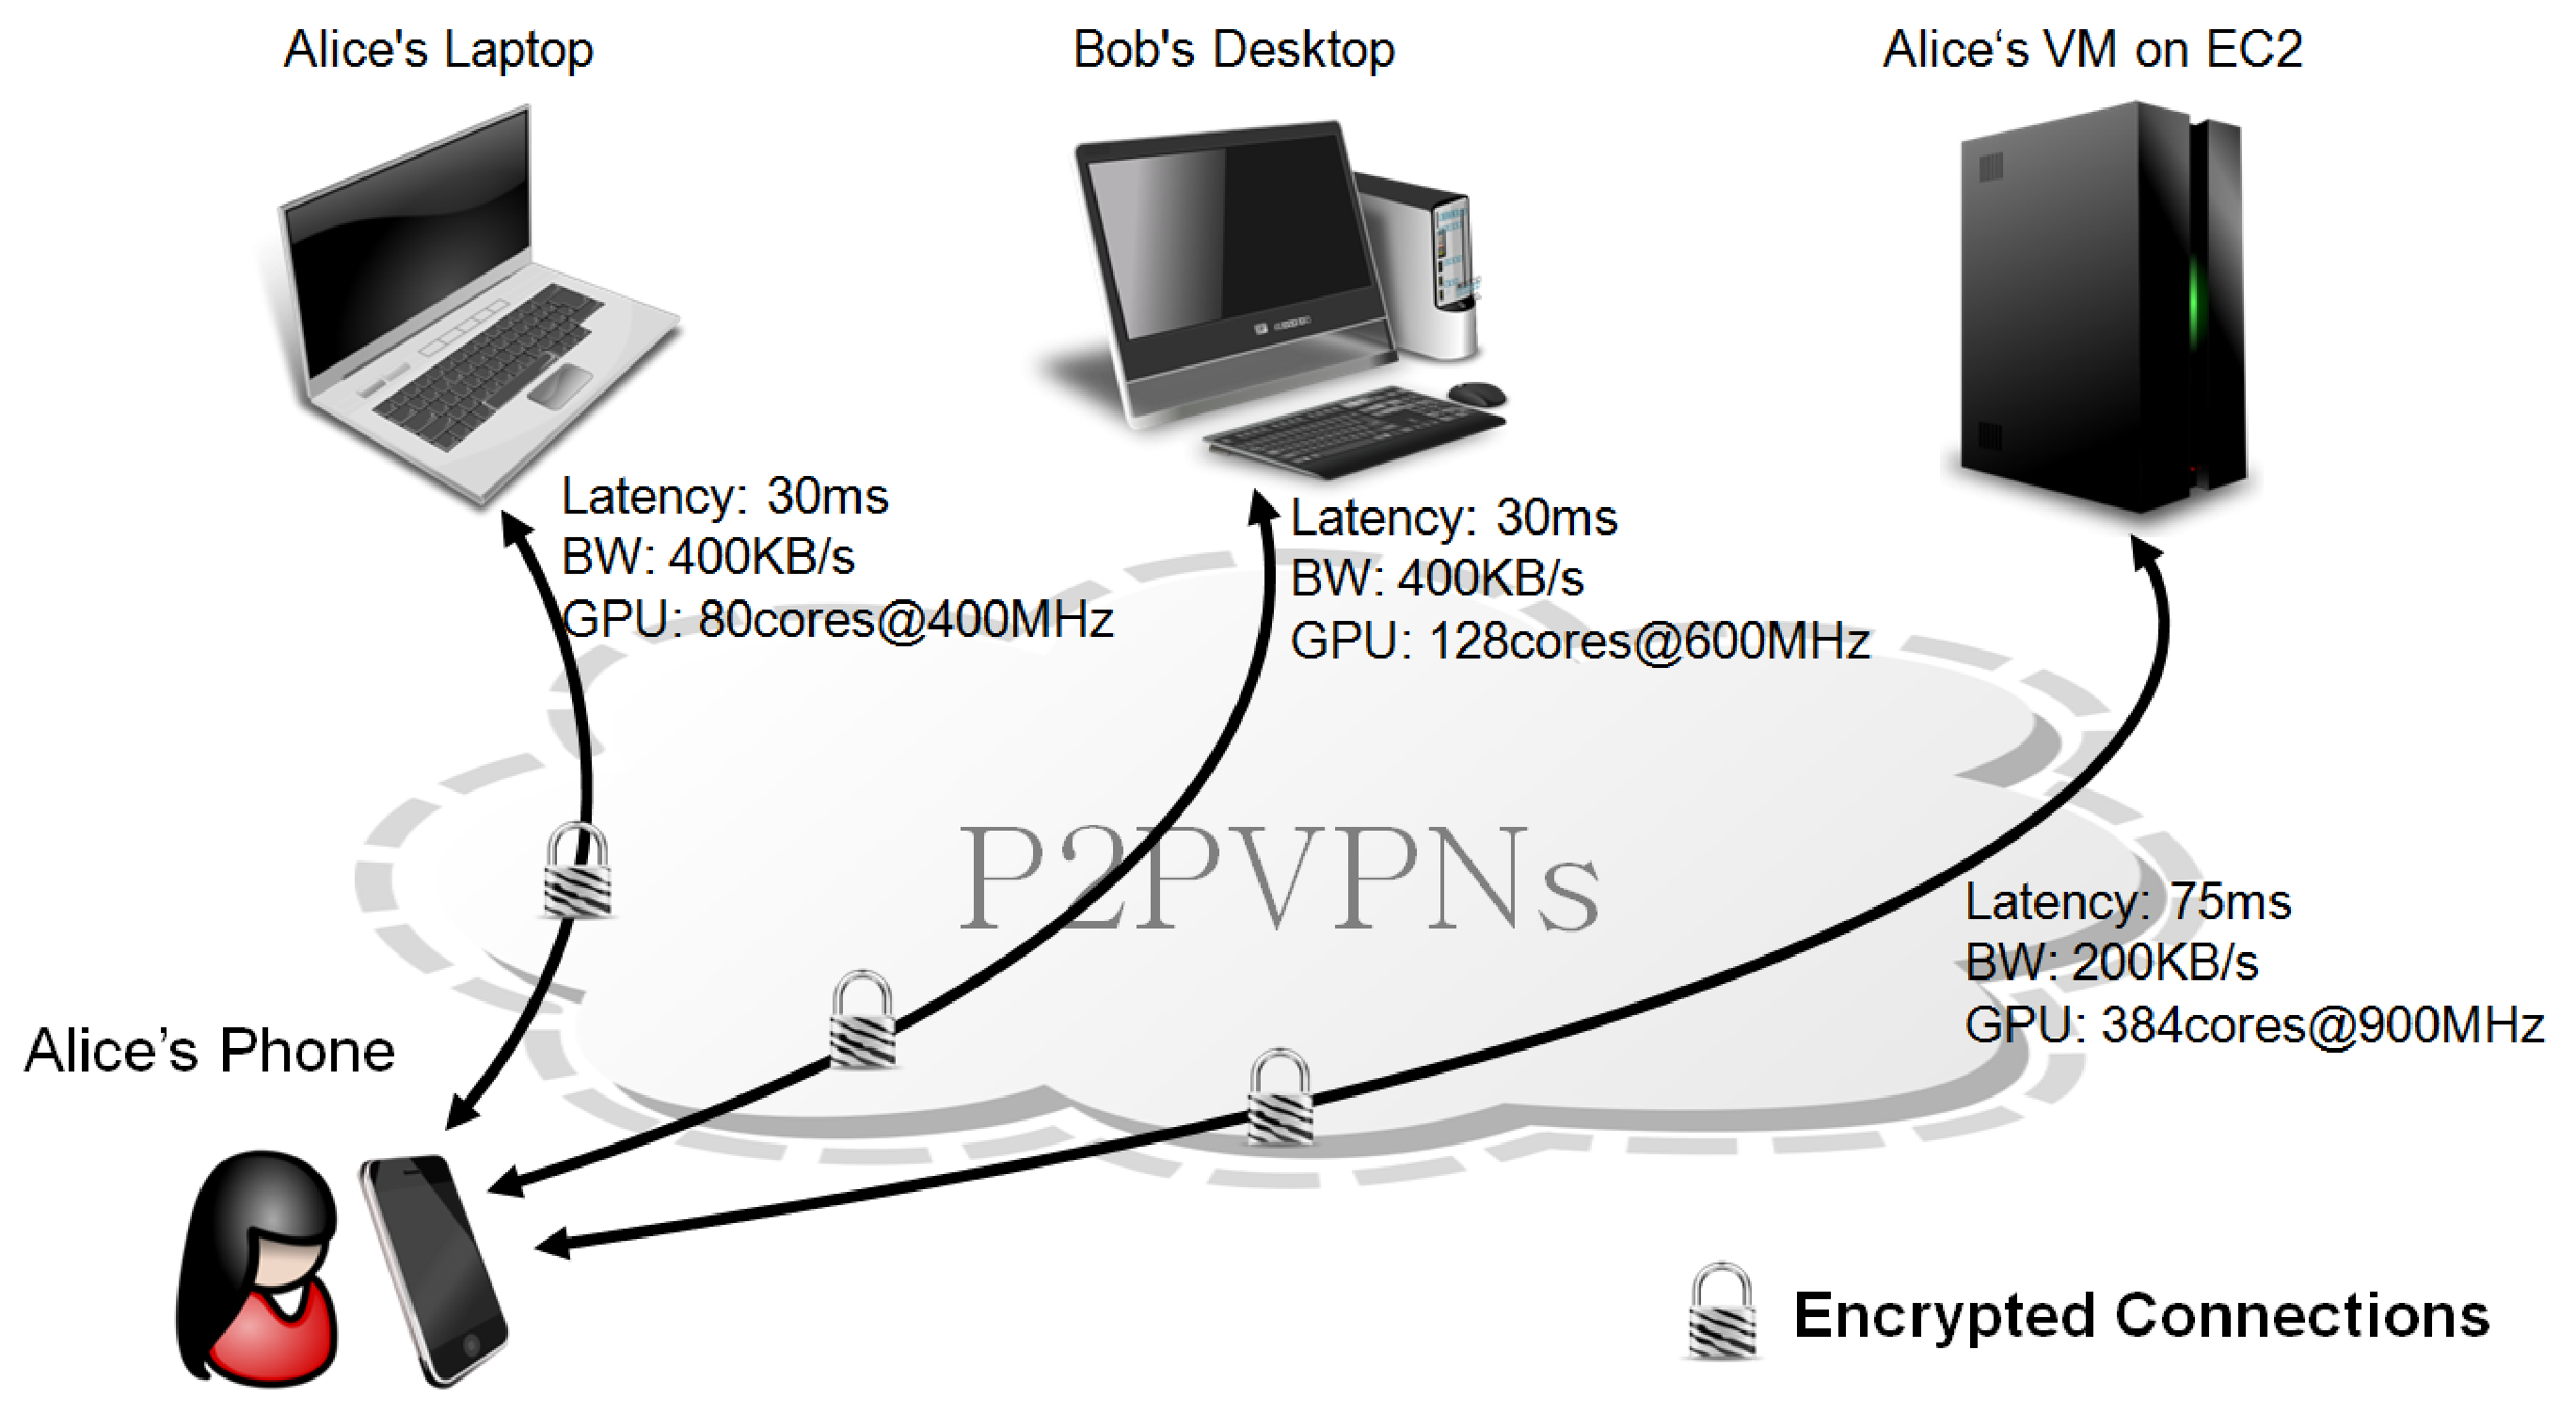
\epsfig{file=figs/motivation.eps, width=5.5in}
\caption{Private networking and node selection}
\label{fig:motivation}
\end{figure}
%
Here is another example of how a developer might take advantage of
OpenCL and the proposed platform in a seamless fashion.
%
Consider a typical facial recognition application in a mobile device
used as a security feature, or for tagging friends on a social
networking application.
%
First, the developer utilizes a CPU implementation.
%
However, the developer quickly realizes the processing limitations of
doing image processing on the CPU and decides that such a workload is
better suited for the GPU or another hardware-based accelerator.
%
With this realization, the developer writes an OpenCL-based
implementation due to its wide support and adoption.
%
Using OpenCL, the developer is able to offload the computation from the
mobile CPU to the mobile GPU and therefore achieve better performance
with less battery consumption.\\
%
The proposed framework aims to extend the umbrella of heterogeneous
computing to include devices beyond the physical host platform.
%
By recompiling the application to link with the proposed framework, the
developer can transparently access remote resources available via the
SocialVPN, including GPUs running on computing resources more powerful
than a mobile device.
%
For instance, if the mobile device is connected to a virtual network
consisting of an Amazon EC2 GPU instance, and the user's personal
workstation, the extensions to the OpenCL framework will automatically
select the best candidate based on available device capabilities, and
network conditions as the target compute node for remote execution.
%
Also, the use of SocialVPN, ensures that computation is offloaded
securely to socially trusted nodes.
%
This enhancement occurs transparently to the developer and the user
requiring only code recompilation. 
%

\section{Contributions}
\label{intro:contributions}
The key contributions of this dissertation can be summarized as
follows:\\
%
{\bf Novel framework for remote computation offloading.} The primary
contribution is a novel framework which addresses the challenge of
remote computation offloading to resources in the cloud the paradigm of
extended hardware-layer heterogeneous computing.
%
Heterogeneous computing uses specialized hardware accelerators to
increase computing throughput and performance.
%
The proposed framework combines the power of cloud offloading with the
flexibility of heterogeneous architecture which expands the dynamic
execution range of mobile platforms, which are typically restricted by
power constraints.\\
%
{\bf Decentralized resource discovery mechanism.} Second
contribution of this proposal is a distributed method of resource
management which handles service discovery, access control, and data
privacy.
%
Previous mobile offloading solutions have not investigated a service
discovery mechanism by assuming the availability of remote computing
resources with static endpoints.
%
The proposed framework advocates a dynamic approach where candidate
computing nodes are discovered at runtime while allowing for a more
flexible design.
%
By using IP multicast-based discovery, the proposed system periodically
locates computing nodes which are available within their social device
network.\\
%
{\bf Workloads characterization using computation to communication
ratio.} 
%
I characterize mobile workloads for the suitability of offloading from
the perspective of {\it Computation to Communication ratio} which is
calculated by the time for workloads to be executed locally divided by
the data transfer time for remote offloading.
%
Thus, in this work, computation to communication ratio for mobile
workloads is a comprehensive measurement which mirrors three dynamic
parameters such as the volume of computation of workloads, the amount of
data to be transferred, and the network conditions.\\
%
{\bf Machine learning-based runtime scheduler.} Prior studies have
primarily focused on core mechanisms for offloading.
%
However, adaptive scheduling in such system is important because
offloading effectiveness can be influenced by varying network
conditions, workload requirements, and load at the target device.
%
In this dissertation, a study on the feasibility of applying machine
learning techniques to address the adaptive scheduling problem in mobile
offloading framework is presented as a third contribution.
%
By taking the algorithm complexity and scheduling performance into
account, a few machine learning algorithms are selected to implement
offline runtime schedulers for mobile offloading framework.
%
Furthermore, I extend the offline machine learning-based runtime
scheduler to the mobile offloading scheduler with online machine
learning techniques.
%
This extension provides an online training mechanism for the machine
learning-based runtime scheduler such that it supports a policy that
dynamically adapts scheduling decisions at runtime based upon the
observation of previous offloading decision and their correctness.\\
%
The prototype implementation of the proposed framework is evaluated,
with regard to end-to-end application performance and energy consumption
in mobile devices, through a variety of network configurations
representing local and wide area network, and various levels of remote
computing capabilities such as typical CPUs, GPUs as well as Amazon EC2
instances.
%
\section{Outline}
\label{intro:outline}
The rest of the proposal is outlined as follows.
%
Chapter 2 provides the necessary background and context for this
proposal.
%
Chapter 3 presents the key idea of extending an OpenCL standard to
support remote offloading framework and integrating the OpenCL API with
RPC-based remote service.
%
Also, in Chapter 3, the decentralized resource discovery mechanism
through a peer-to-peer virtual private network is presented.
%
Chapter 4 characterizes mobile workloads the perspective of computation
to communication ratio.
%
Also, Chapter 5 explains machine learning techniques for a runtime
scheduler for remote offloading system.
%
Chapter 6 describes an online training mechanism for machine
learning-based mobile offloading scheduler.
%
Then, Chapter 7 introduces a proximity-aware clustering system which can
lead an additional performance improvement in conjunction with mobile
offloading framework.
%
Lastly, in Chapter 8, the dissertation is summarized and future work
is detailed.
%
